\scanpage{23}
are isomorphic to subgroups of the group of exterior automorphisms of $\mathrm{G}$) ?

In a different direction, it would 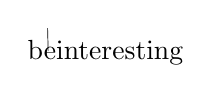
\begin{tikzpicture}[baseline=(w.base),x=1em,y=1ex]
\node[anchor=base west,inner sep=0pt] (w) at (0,0) {beinteresting};
\draw[line width=.25pt] (.76,.72) -- (.74,2.65);
\end{tikzpicture} to know more about the canonical morphism $\underline{\mathrm{g}}\handwritten{\longrightarrow}\underline{\mathrm{h}}/\mathrm{W}$, where $\underline{\mathrm{g}}$ is the Lie algebra of $\mathrm{G}$ and $\underline{\mathrm{h}}$ a Cartan subalgebra, and of the orbits of $\mathrm{G}$ on $\underline{\mathrm{g}}$, and the analoguous morphism of Steinberg $\mathrm{G}\handwritten{\longrightarrow}\mathrm{T}/\mathrm{W}$ and the orbits of $\mathrm{G}$ acting on itself. Do you know for instance exactly how varies the rank (= rang of the tangent map) of this \deleted{applic\unsure{at}i} map ? There are some reasons to believe that \deleted{this} for points of unipotent orbits of 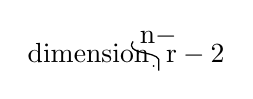
\begin{tikzpicture}[baseline=(d.base),x=1em,y=1ex]
\node[anchor=base west,inner sep=0pt] (d) at (0,0) {dimension};
\node[anchor=base west,inner sep=0pt] at (5.0,0) {$\mathrm{r}-2$};
\node[anchor=base west,inner sep=0pt] at (4.05,1.6) {$\inserted{\mathrm{n}-}$};
\draw[line width=.45pt] (3.83,1.8) .. controls (3.5,.7) and (4.65,1.0) .. (4.76,.28) -- (4.76,-.65);
\fill (4.57,-.26) circle[radius=.035em];
\end{tikzpicture} (just 
\begin{tikzpicture}[baseline=(live.base),x=1em,y=1ex]
\node[anchor=base west,inner sep=0pt] at (0,1.05) {\deleted{the next lower after}};
\node[anchor=base west,inner sep=0pt] (live) at (0,0) {\inserted{the next lower after}};
\end{tikzpicture} the maximal dimension $\mathrm{n}-\mathrm{r}$), the rank is $\mathrm{r}-1$ in case all roots have same length (that is the corresponding diagrams $\mathrm{A}_{\unsure{\begin{tikzpicture}[baseline=(r.base),x=1em,y=1ex]\node[inner sep=0pt] at (0,0) {$\scriptstyle\mathrm{n}$};\node[inner sep=0pt] (r) at (.025,.03) {$\scriptstyle\mathrm{r}$};\end{tikzpicture}|\mathbb{r}}},\mathrm{D}_{\unsure{\begin{tikzpicture}[baseline=(r.base),x=1em,y=1ex]\node[inner sep=0pt] at (0,0) {$\scriptstyle\mathrm{n}$};\node[inner sep=0pt] (r) at (.04,.04) {$\scriptstyle\mathrm{r}$};\end{tikzpicture}|\mathbb{r}}},\mathrm{E}_{\handwritten{6}},\mathrm{E}_{\handwritten{7}},\mathrm{E}_{\handwritten{8}}$ are those corresponding to Klein singularities), and $\handwritten{<}\mathrm{r}-1$ in 
\begin{tikzpicture}[baseline=(other.base),x=1em,y=1ex]
\node[anchor=base west,inner sep=0pt] (other) at (.3,0) {other};
\node[anchor=base west,inner sep=0pt] at (.10,1.55) {\inserted{\handwritten{all}}};
\draw[line width=.3pt] (0,-.1) .. controls (.25,1.15) and (1.62,.68) .. (1.8,1.4);
\end{tikzpicture} cases; in the first case, I would expect that there is just one orbit as stated, by the way, and maybe this property will be caracteristic of the ``homogene\deleted{a}ous'' case when all roots have same length. Also, what can be said of the dim\unsure{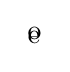
\begin{tikzpicture}[baseline=(e.base),x=1em,y=1ex]\node[inner sep=0pt] (e) at (0,0) {e};\node[inner sep=0pt] at (.02,.34) {o};\end{tikzpicture}|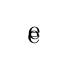
\begin{tikzpicture}[baseline=(e.base),x=1em,y=1ex]\node[inner sep=0pt] (e) at (0,0) {e};\node[inner sep=0pt] at (.02,.34) {e};\end{tikzpicture}}nsion of the set of all Borel subgroups containing a given element $\mathrm{g}\handwritten{\in}\mathrm{G}$, resp. whose Lie algebra contains a given element $\mathrm{x}\handwritten{\in}\underline{\mathrm{g}}$ ? If $2\mathrm{N}=\mathrm{n}-\mathrm{r}$ is the number of roots and if the dimension of the orbit of the given element is $2\mathrm{N}-2\mathrm{i}$, I would expect the dimension of the previous variety to be equal to $\mathrm{i}$; the inequality $\handwritten{\leqslant}\mathrm{i}$ would imply, by generalizing a depth argument of Br\unsure{
\begin{tikzpicture}[baseline=(i.base),x=1em,y=1ex]\node[inner sep=0pt] at (0,0) {e};\node[inner sep=0pt] (i) at (-.025,.025) {i};\end{tikzpicture}}\unsure{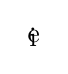
\begin{tikzpicture}[baseline=(e.base),x=1em,y=1ex]\node[inner sep=0pt] at (0,0) {i};\node[inner sep=0pt] (e) at (.025,.025) {e};\end{tikzpicture}}skorn, that the singularities of the fibers of your map $\underline{\mathrm{g}}\handwritten{\longrightarrow}\underline{\mathrm{h}}/\mathrm{W}$ (resp. Steinberg's $\mathrm{G}\handwritten{\longrightarrow}\mathrm{T}/\mathrm{W}$ in case $\mathrm{G}$ is simply connected instead of adjoint) are ``rational'', i.e. i\unsure{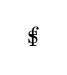
\begin{tikzpicture}[baseline=(f.base),x=1em,y=1ex]\node[inner sep=0pt] at (0,0) {s};\node[inner sep=0pt] (f) at (0,.025) {f};\end{tikzpicture}} $\mathrm{F}$ is such a fiber and $\mathrm{F}'\overset{\mathrm{f}}{\handwritten{\longrightarrow}}\mathrm{F}$ a resolution of singularities of $\mathrm{F}$, t\unsure{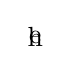
\begin{tikzpicture}[baseline=(h.base),x=1em,y=1ex]\node[inner sep=0pt] at (0,0) {e};\node[inner sep=0pt] (h) at (0,.015) {h};\end{tikzpicture}}\unsure{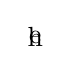
\begin{tikzpicture}[baseline=(e.base),x=1em,y=1ex]\node[inner sep=0pt] at (0,0) {h};\node[inner sep=0pt] (e) at (0,.015) {e};\end{tikzpicture}}n $\mathrm{R}^{\mathrm{i}}\mathrm{f}_{\handwritten{*}}(\underline{\mathrm{O}}_{\mathrm{F}'}^{\deleted{\unsure{\mathrm{t}|*}}})=0$ for $\mathrm{i}\handwritten{>}0$. Maybe the ans\unsure{
\begin{tikzpicture}[baseline=(w.base),x=1em,y=1ex]\node[inner sep=0pt] (w) at (0,0) {w};\draw[line width=.35pt] (-.27,.63) -- (-.25,-.38) .. controls (0,-.57) and (.23,-.43) .. (.25,-.30) -- (.25,.58);\end{tikzpicture}|u}\begin{tikzpicture}[baseline=(e.base),x=1em,y=1ex]\node[inner sep=0pt] (e) at (0,0) {e};\draw[line width=.35pt] (-.22,.02) -- (-.22,1.10);\end{tikzpicture}r \deleted{\unsure{ot|to}}\handwritten{to} most of the questions I am asking are well known and I am just ignorant; for some of them, it would indeed be scandalous that the experts do not know the answer ! In any case, I would be grateful for any comment you would have on any of my questions.

\figure{\begin{tikzpicture}[x=1cm,y=1cm]
\node[anchor=base west,inner sep=0pt] at (0,0) {Sincerely yours};
\node[anchor=base west,inner sep=0pt] at (7.0,-.55) {\handwritten{A\,G\unsure{rothendieck}}};
\fill (7.93,-.32) circle[radius=.012cm];
\node[inner sep=0pt] at (8.48,-1.85) {\unsure{\begin{tikzpicture}[x=1cm,y=1cm]
\draw[line width=.25pt] (0,.48)--(0,.41);
\draw[line width=.25pt] (0,.38)--(0,.29);
\draw[line width=.25pt] (-.005,.25)--(-.005,.18);
\draw[line width=.25pt] (0,.16)--(-.005,.07);
\draw[line width=.25pt] (-.005,.05)--(-.005,-.02);
\end{tikzpicture}}};
\end{tikzpicture}}
% The raised line above the e in beinteresting has no assigned textual function.
% Raised n- is definite; typewritten versus pen medium remains uncertain. Its leader and the separate low point are drawn.
% Mixed typewriter impressions are overlaid without assigning an unattested strike order.
% A detached point above the early signature strokes is retained without assigning punctuation.
% The separate interrupted bottom trace is drawn; ink versus surface origin and function remain uncertain.
% archive sheet number: 22
